\documentclass[a4paper,12pt]{article}
\usepackage{amssymb}
\usepackage{amsmath}
\usepackage[utf8]{vietnam}
\usepackage{geometry}
\usepackage{tcolorbox}
\usepackage{graphicx}
\usepackage{lipsum}
\usepackage{pifont}
\usepackage{ragged2e}
\usepackage{setspace}
\usepackage{tocloft}
\usepackage{titlesec}
\usepackage{xcolor}
\usepackage{listings}

\usepackage{fancyhdr}
\setlength{\headheight}{32pt}
\addtolength{\topmargin}{-16pt}
\usepackage{caption}
\usepackage{tabularx}
\usepackage{booktabs}
\usepackage{enumitem}
\usepackage{placeins}
\usepackage[colorlinks=true, urlcolor=blue, hidelinks]{hyperref}
\usepackage{tikz}
\usetikzlibrary{shapes.geometric, arrows.meta, positioning, fit, backgrounds}
\usepackage{booktabs,tabularx,array,tikz,graphicx}

\pagestyle{fancy}
\fancyhf{}
\fancyhead[R]{\ifnum\value{page}>2 \vspace*{0.4cm} \textit{Intro to AI -- Wrongway Quoridor Agent}\hspace{-2.3cm} \fi}
\fancyhead[L]{\ifnum\value{page}>2 \raisebox{-1ex}{\makebox[\textwidth]{\hrulefill}} \fi}
\fancyfoot[C]{\ifnum\value{page}>2 \thepage \fi}

\renewcommand{\headrulewidth}{0pt}

\geometry{left=2.5cm,right=2cm,top=2.2cm,bottom=2.2cm}
\sloppy
\newtcbox{\inlinecode}{on line,
	boxsep=1pt, left=1pt, right=1pt, top=1pt, bottom=1pt,
	colframe=gray!80, colback=gray!20,  
	boxrule=0.5pt, arc=3pt,
	nobeforeafter}
\lstset{
	language=Python,                      
	basicstyle=\ttfamily\footnotesize,
	keywordstyle=\color{blue!80!black},
	commentstyle=\color{gray!90!black}, 
	stringstyle=\color{red!70!black},          
	numbers=left,  
	numberstyle=\tiny\color{black!60},
	backgroundcolor=\color{black!3},
	frame=single,
	tabsize=4,
	breaklines=true,
	captionpos=b,
	columns=fixed, 
	basewidth=0.5em,
}

\begin{document}
	
\begin{titlepage}
    \thispagestyle{empty}
    % Double-line decorative border (HCMUS thesis & project standard)
    \begin{tikzpicture}[remember picture, overlay]
        \draw[line width=1.8pt, black] 
            ([xshift=22mm, yshift=-18mm]current page.north west) 
            rectangle 
            ([xshift=-16mm, yshift=18mm]current page.south east);
        \draw[line width=0.6pt, black] 
            ([xshift=24mm, yshift=-20mm]current page.north west) 
            rectangle 
            ([xshift=-18mm, yshift=20mm]current page.south east);
        % Subtle decorative corner lines
        \draw[line width=0.4pt, black] 
            ([xshift=25mm, yshift=-21mm]current page.north west) -- ++(10mm, 0);
        \draw[line width=0.4pt, black] 
            ([xshift=25mm, yshift=-21mm]current page.north west) -- ++(0, -10mm);
        \draw[line width=0.4pt, black] 
            ([xshift=-19mm, yshift=-21mm]current page.north east) -- ++(-10mm, 0);
        \draw[line width=0.4pt, black] 
            ([xshift=-19mm, yshift=-21mm]current page.north east) -- ++(0, -10mm);
        \draw[line width=0.4pt, black] 
            ([xshift=25mm, yshift=21mm]current page.south west) -- ++(10mm, 0);
        \draw[line width=0.4pt, black] 
            ([xshift=25mm, yshift=21mm]current page.south west) -- ++(0, 10mm);
        \draw[line width=0.4pt, black] 
            ([xshift=-19mm, yshift=21mm]current page.south east) -- ++(-10mm, 0);
        \draw[line width=0.4pt, black] 
            ([xshift=-19mm, yshift=21mm]current page.south east) -- ++(0, 10mm);
    \end{tikzpicture}

    \begin{center}
        \vspace*{0.2cm}
        {\fontsize{13pt}{16pt}\selectfont \textbf{VIETNAM NATIONAL UNIVERSITY HO CHI MINH CITY}}\\[4pt]
        {\fontsize{13pt}{16pt}\selectfont \textbf{UNIVERSITY OF SCIENCE}}\\[4pt]
        {\fontsize{12pt}{15pt}\selectfont \textbf{FACULTY OF INFORMATION TECHNOLOGY}}\\[5pt]
        {\fontsize{11pt}{14pt}\selectfont \textbf{ADVANCED PROGRAM IN COMPUTER SCIENCE (APCS)}}\\[8pt]
        \noindent\rule{0.45\textwidth}{0.8pt}\\[0.6cm]
        
        
\includegraphics[width=4.2cm]{logo.png}\\[0.6cm]
        
        {\fontsize{13pt}{16pt}\selectfont \textbf{COURSE PROJECT REPORT}}\\[5pt]
        {\fontsize{12pt}{15pt}\selectfont \textbf{CS420 -- INTRODUCTION TO ARTIFICIAL INTELLIGENCE}}\\[0.8cm]
        
        \begin{tcolorbox}[
            colback=white,
            colframe=black,
            arc=0mm,
            boxrule=1.5pt,
            width=0.92\textwidth,
            halign=center
        ]
            \vspace{0.25cm}
            {\fontsize{17pt}{22pt}\selectfont \textbf{WRONGWAY QUORIDOR AGENT}}\\[8pt]
            {\fontsize{11.5pt}{16pt}\selectfont \textbf{High-Performance Game-Theoretic Search, SPSA AI Tuning Pipeline, and Tournament Evaluation}}
            \vspace{0.25cm}
        \end{tcolorbox}
        
        \vfill
        
        \begin{minipage}{0.84\textwidth}
            \renewcommand{\arraystretch}{1.35}
            \begin{tabular}{@{}ll@{}}
                \textbf{Group Members:} & \textbf{Student ID:} \\
                \quad \textbf{Phạm Hữu Nam} (Team Leader) & \quad \textbf{24125015} \\
                \quad \textbf{Bùi Nguyễn Đức Trọng} & \quad \textbf{24125021} \\
                \quad \textbf{Nguyễn Hoàng Thuận Phát} & \quad \textbf{24125072} \\
                \quad \textbf{Vũ Quốc Lâm} & \quad \textbf{23125011} \\
            \end{tabular}
        \end{minipage}
        
        \vfill
        \vspace*{0.3cm}
        {\fontsize{11pt}{14pt}\selectfont \textbf{TP. HỒ CHÍ MINH, THÁNG 11/2026}}\\[0.1cm]
    \end{center}
\end{titlepage}

\newpage
    
    \renewcommand{\baselinestretch}{1.05}\normalsize
    \tableofcontents
    \renewcommand{\baselinestretch}{1.15}\normalsize

	\newpage

\section{Project Overview \& Core Ideas}

\subsection{Quoridor Game Specifications and Constraints}
Quoridor is an adversarial, two-player zero-sum abstract strategy game played on a $9 \times 9$ grid. Each player begins with a pawn situated at their starting baseline and a reserve of $10$ walls. The primary objective is to maneuver one's pawn across the board to any cell in the opponent's starting row before the opponent accomplishes the reverse:
\begin{itemize}[leftmargin=1.5em]
    \item \textbf{Player 0 (P0):} Starts at coordinate $[8, 4]$ (bottom row) and aims to reach row $0$. Player 0 moves first.
    \item \textbf{Player 1 (P1):} Starts at coordinate $[0, 4]$ (top row) and aims to reach row $8$. Player 1 moves second.
\end{itemize}

On each turn, an agent must execute exactly one of three actions within a strict execution deadline of \textbf{1.000 second}:
\begin{enumerate}[leftmargin=1.5em]
    \item \textbf{Move Pawn:} Advance one orthogonal step to an adjacent cell through an open edge. When adjacent to the opponent pawn and unblocked, the pawn can jump straight over; if blocked behind the opponent by a wall or board border, diagonal hops are permitted.
    \item \textbf{Place Wall:} Position a $2$-unit wall horizontally ($H$) or vertically ($V$) along the grid grooves. Walls cannot overlap, intersect, or completely seal off either player's path to their respective goal baseline.
    \item \textbf{Pass:} Forfeit the active turn (effectively an emergency fallback).
\end{enumerate}

The match is terminated as a victory as soon as a pawn steps onto its target goal row, or declared a draw if neither player wins within $500$ collective turns. Any action exceeding the $1.0\text{s}$ time limit, raising an unhandled exception, or attempting an illegal move forfeits the active turn.

\subsection{Origin of Benchmark Opponents \& the \texttt{wrongway.app} Suite}
To evaluate our agent against diverse, competitive tactics rather than simple static heuristics, our team established an external sparring framework interfaced directly with the official competitive web platform \textbf{\texttt{wrongway.app}}. We extracted and wrapped the production JavaScript engine from \texttt{wrongway.app} via Node.js IPC to create a comprehensive test suite of five distinct play styles:
\begin{itemize}[leftmargin=1.5em]
    \item \textbf{\texttt{web\_bot\_hard} (Mauerer Style):} The official web hard bot utilizing an advanced Alpha-Beta search engine focused on aggressive blockade building and corridor chokes.
    \item \textbf{\texttt{web\_bot\_renner} (Runner Style):} An ultra-aggressive pure speedrun rusher ($VD = 40, WB = -40$) that hoards walls exclusively for game-ending lines.
    \item \textbf{\texttt{web\_bot\_konter} (Counter-Puncher Style):} A balanced, highly tactical engine operating with zero artificial wall bias ($WB = 0, VD = 0$), maintaining path flexibility and punishing premature commitments.
    \item \textbf{\texttt{web\_bot\_chameleon} (Adaptive Multi-Style):} An anti-overfitting bot that randomly shifts core styles and applies dynamic weight jittering ($\pm 8\%$) every match.
    \item \textbf{\texttt{web\_bot\_grandmaster} (Deep Search Engine):} A deep Alpha-Beta engine with a $650,000$ node budget, expanded candidate branching, and multi-step trap defense ($XP = 3$).
\end{itemize}
Along with elite peer agents developed by other student teams (e.g., \texttt{trong\_mcts\_frontier\_combined\_v5} and \texttt{24125015\_improve\_bigbook}), this diverse suite provided our primary training gauntlet.

\subsection{Key Ideas Behind Agent 24125015}
Our agent's development began with a basic Negamax search and simple distance differences. However, initial wall generation was terribly slow and naive, causing shallow search and frequent tactical blindness. Through reverse-engineering insights from \texttt{web\_bot\_hard} and extensive AI parameter tuning, we synthesized Agent \texttt{24125015} (the \textit{v10 Ultimate Hybrid Engine}) based on six foundational pillars:
\begin{enumerate}[leftmargin=1.5em]
    \item \textbf{Incremental Bitboard Engine ($O(1)$ 2-XOR):} All 81 board cells and directional edge connections are represented as 81-bit integer masks. Adding or removing a wall requires exactly one bitwise XOR operation per cardinal direction, eliminating Python object allocation and achieving high throughput during tree search.
    \item \textbf{Horizontal-Mirror Canonical Zobrist Symmetries:} Every board state is mapped to its horizontal reflection across column $c = 4$. Transposition Table (TT), wall caches, and distance caches index only the canonical symmetry, halving memory usage and unifying symmetrical opening and endgame positions.
    \item \textbf{Iterative Deepening Negamax with PVS \& Safe LMR:} The search tree is explored via Principal Variation Search (PVS) with strict null-window refutations for non-PV moves. Non-tactical wall moves late in candidate order ($\text{wall\_i} \ge 3$) are pruned via Late Move Reductions (LMR), while big distance-gain walls ($\Delta d \ge 3$) and bottleneck closures are strictly protected.
    \item \textbf{Endgame 0-Wall Cutoffs:} When both players exhaust their walls ($\text{barr} = [0, 0]$), a path lead of $\ge 3$ steps immediately returns a decisive score in $O(1)$, while completing depth 18 in iterative deepening serves as a computational stopping threshold to save CPU budget.
    \item \textbf{Leaf Trap Potential ($\text{potential}()$):} Leaf evaluations calculate virtual single-wall detour expansions ($KS = 1$), penalizing positions where the opponent can force our pawn into a corridor detour, with 2-wall extensions preserved from earlier experiments.
    \item \textbf{Calibrated Root Bias \& Sidestep Tie-Breaker:} Inspired by the \textit{Konter} style of \texttt{web\_bot\_hard}, eliminating artificial wall subsidies ($WB = 0.0, VD = 12.0, NM = 0.0$) and adding a lateral sidestep bonus ($\text{side\_i} = 4000$) allows P1 to naturally break opponent flank attacks via sideways steps to $(3,3)$ or $(3,5)$, preserving all 10 walls and converting P1 into an effective counter-attacking defense.
\end{enumerate}


\section{Agent Architecture \& Search Engine}

\subsection{Bitboard Representation and $O(1)$ Edge Mask Manipulation}
Conventional game engines represent the Quoridor board using Python nested lists or graphs, incurring severe reference chasing and object allocation penalties. Agent \texttt{24125015} models all state variables using native 81-bit integer bitboards:
\begin{itemize}[leftmargin=1.5em]
    \item \textbf{Cell Coordinates:} Cell $(r, c)$ corresponds to bit $u = 9r + c \in [0, 80]$. Constants $\text{ROW}[r] = ((1 \ll 9) - 1) \ll 9r$ and $\text{ALL} = (1 \ll 81) - 1$ provide constant-time mask operations.
    \item \textbf{Directional Connectivity Masks:} Movement connectivity across adjacent cells is maintained via four 81-bit integer masks: $\text{mD}$ (step down), $\text{mU}$ (step up), $\text{mR}$ (step right), and $\text{mL}$ (step left).
    \item \textbf{$O(1)$ 2-XOR Incremental Updates:} When placing or unplacing a wall index $w$, edge masks are updated instantaneously via bitwise XOR without allocations:
    \begin{equation}
        \text{mD} \leftarrow \text{mD} \oplus \text{WM\_D}[w], \quad \text{mU} \leftarrow \text{mU} \oplus \text{WM\_U}[w]
    \end{equation}
    where $\text{WM\_D}[w]$ and $\text{WM\_U}[w]$ are precomputed static bitmasks representing the blocked groove edges.
    \item \textbf{Fast Bitwise BFS:} Shortest paths to target baselines are computed via bitwise flood-fill. The open frontier $F$ expands through bit shifts:
    \begin{equation}
        F_{\text{next}} = ((F \& \text{mD}) \ll 9) \mid ((F \& \text{mU}) \gg 9) \mid ((F \& \text{mR}) \ll 1) \mid ((F \& \text{mL}) \gg 1)
    \end{equation}
    This bitwise BFS executes up to $10\times$ faster than Dijkstra, computing distances in under $8\mu\text{s}$.
\end{itemize}

\subsection{Mirror-Canonical Symmetries \& Specialized Caching}
Quoridor possesses an exact reflective symmetry along the vertical axis (column $c = 4$). For any board state with wall configuration $W$ and pawn positions $p_{\text{me}}, p_{\text{op}}$, reflecting all columns across the center ($c' = 8 - c$) produces an isomorphic game state.

Our engine utilizes tailored representations for its high-performance caches:
\begin{itemize}[leftmargin=1.5em]
    \item \textbf{Transposition Table ($\text{TT}$), $\text{wcache}$, and $\text{xcache}$:} Indexed using 64-bit mirror-canonical Zobrist keys. Random bitstrings are generated for pawn positions $\text{ZP}$, mirrored positions $\text{ZPM}$ ($\text{ZPM}[s][u] = \text{ZP}[s][\text{mir}(u)]$), wall slots $\text{ZW}$, mirrored walls $\text{ZWM}$, wall counters $\text{ZB}$, and turn key $\text{ZT}$. The canonical key is $K_{\text{canon}} = \min(K, K_m)$.
    \item \textbf{Leaf Potential Cache ($\text{pcache}$):} Indexed directly by canonical wall bitmask and mirrored target pawn: $ck = (W_{\text{canon}} \ll 8) \mid (p_{\text{canon}} \ll 1) \mid a$.
    \item \textbf{Single-Player Distance Cache ($\text{dcache}$):} Indexed by wall configuration bitmask, pawn cell, and target goal baseline: $(W \ll 7) \mid (p \ll 1) \mid g$.
\end{itemize}
This granular caching strategy eliminates redundant calculations across symmetric lines while avoiding unnecessary hashing overhead.

\subsection{Iterative Deepening Negamax with PVS and Safe LMR}
Search is organized as an iterative deepening framework, expanding search horizons ply-by-ply from depth $1$ upwards within the dynamic time budget.
\begin{itemize}[leftmargin=1.5em]
    \item \textbf{Principal Variation Search (PVS):} The root move ordering ranks moves based on previous iteration PV scores, history heuristics, and heuristic wall gain metrics. The principal variation candidate is evaluated with a full window $(\alpha, \beta)$. All alternative candidate moves are initially tested with a minimal null-window $(\alpha, \alpha + 1)$. A full re-search is triggered only when a null-window probe fails high ($score > \alpha$).
    \item \textbf{Stockfish-Style Partial Iteration Adoption:} When the hard time limit ($T_{\text{hard}} = 0.80\text{s}$) interrupts search mid-iteration, the engine adopts the partial result if and only if a newly completed candidate move has proven to be strictly superior to Move 0 ($best\_done \neq r_0$). Otherwise, it falls back to the fully verified previous iteration, preventing partial-subset tactical blunders.
    \item \textbf{Tactical Late Move Reductions (LMR):} Wall moves evaluated later in candidate order at non-PV nodes are conditionally reduced to accelerate tree traversal. The exact reduction predicate implemented is:
    \begin{align}
        \text{do\_lmr} = (\text{opp\_has\_walls} &\land \neg\text{is\_pv} \land \text{depth} \ge 3 \land \text{wall\_i} \ge 3 \nonumber \\
        &\land d_{\text{op}} > 2 \land \Delta d_{\text{op}} < 3 \land \text{idx} \notin \{k_1, k_2\})
    \end{align}
    When active, the reduction depth is:
    \begin{equation}
        \text{red} = \begin{cases}
            2 & \text{if } \text{depth} \ge 5 \land \text{wall\_i} \ge 6 \\
            1 & \text{otherwise}
        \end{cases}
    \end{equation}
    Crucially, LMR is bypassed if: (1) the opponent has 0 walls ($\text{opp\_has\_walls} = \text{False}$), preserving exact endgame conversion; (2) the opponent is within 2 steps of their goal ($d_{\text{op}} \le 2$); (3) the wall gains a major distance advantage ($\Delta d_{\text{op}} = n_O - d_O \ge 3$); or (4) the candidate matches killer moves $k_1, k_2$.
\end{itemize}

\subsection{Endgame 0-Wall Cutoffs \& Search Horizon Management}
When both players exhaust their wall supply ($\text{barr} = [0, 0]$), no further barriers can be placed on the board, and the game transitions into a pure pawn race on the existing static grid topology. Agent \texttt{24125015} manages this phase through two complementary mechanisms:
\begin{enumerate}[leftmargin=1.5em]
    \item \textbf{Interior Distance-Gap Decisive Cutoff:} Inside the recursive search, when $\text{barr} = [0, 0]$, if one player possesses a shortest-path advantage of $\ge 3$ steps ($d_S \le d_O - 3$), the node immediately returns a decisive terminal utility:
    \begin{equation}
        U(S) = \begin{cases}
            +\text{BOT\_WIN} - \text{ply} - 2 d_S & \text{if } d_S \le d_O - 3 \\
            -(\text{BOT\_WIN} - \text{ply} - 2 d_O) & \text{if } d_O \le d_S - 3
        \end{cases}
    \end{equation}
    In typical open board play, jumping over an opposing pawn gains at most 1 step, making a 3-step lead decisive under turn alternation. While intricate labyrinth corridors formed by earlier walls can introduce non-trivial blocking dynamics that warrant further theoretical study, this heuristic cutoff provides powerful tree pruning without observed blunders in practice.
    \item \textbf{Root Iterative Stopping Threshold (Depth 18):} In $\text{choose\_action}()$, if both wall inventories are zero and iterative deepening completes depth $18$ ($\text{completed} \ge 18$), the loop terminates:
    \begin{equation}
        \textbf{if } \text{zero\_walls} \land \text{completed} \ge 18: \textbf{break}
    \end{equation}
    Because pawn-only branching is narrow ($1 \div 4$ moves), continuing deeper iterations yields diminishing returns. Depth 18 functions as a computational stopping threshold that safely preserves CPU time.
\end{enumerate}

\subsection{Heuristic Evaluation Function \& Leaf Trap Potential}
Position scoring at leaf nodes is executed via an integer-scaled model ($\text{evaluate\_int}()$, scaled by $1{,}000$ to avoid floating-point overhead) that synthesizes 16 linear features with endgame adjustments and leaf trap potentials:
\begin{equation}
    \text{Score}_{\text{int}}(S) = \sum_{i=0}^{15} W_i f_i(S) + \text{Adj}_{\text{endgame}} + \text{TieBreakers} + \Delta \text{Trap}(S)
\end{equation}
The primary distance differential is defined as:
\begin{equation}
    \text{diff} = d_{\text{op}} - d_{\text{me}}
\end{equation}
which is positive when our pawn is closer to its goal than the opponent. Beyond the linear feature vector, $\text{evaluate\_int}()$ applies:
\begin{itemize}[leftmargin=1.5em]
    \item \textbf{Endgame Step Race Bonus:} If both wall counts reach zero ($\text{barr} = [0, 0]$), a bonus of $+180{,}000$ (or $-180{,}000$) is applied when $|\text{diff}| \ge 2$, reinforcing decisive race convergence.
    \item \textbf{Geometric Tie-Breakers:} Adds $+2{,}200 \times (\text{prog}_{\text{me}} - \text{prog}_{\text{op}})$ to favor advancement toward the goal baseline, and $-1{,}000 \times (|c_{\text{me}} - 4| - |c_{\text{op}} - 4|)$ to encourage central positioning on equal-length paths.
    \item \textbf{Leaf Trap Potential:} Minimax search can suffer from horizon blindness against corridor traps. The function $\text{potential}(a)$ evaluates the maximum virtual detour that player $a$ can impose on opponent $v = 1 - a$ with a single wall placement ($KS = 1$). The differential trap term is:
    \begin{equation}
        \Delta \text{Trap}(S) = \begin{cases}
            \text{WS} \cdot (\text{pot}(\text{me}) - \text{pot}(\text{op})) & \text{if } \text{WS} > 0 \land (\text{barr}[0] > 0 \lor \text{barr}[1] > 0) \\
            0 & \text{otherwise}
        \end{cases}
    \end{equation}
    Lazy evaluation skips trap computation when the preliminary score falls outside the search window by a margin derived from $\text{LZ} = 9.0$.
\end{itemize}

\subsection{Root Bias Calibration \& Lateral Sidestep Bonus}
A breakthrough in solving the Player 1 disadvantage was the elimination of artificial root subsidies. In earlier versions, placing a wall received an artificial bonus of $WB = +34.48$, while forward moves received $VD = +54.25$. When Player 0 placed an opening flank wall $H(5,0)$, P1 was lured into burning walls defensively ($H(2,3)$ and $V(5,2)$) or stepping forward into dead-end cages.

In Agent \texttt{24125015}, root parameters were recalibrated to $WB = 0.0$, $VD = 12.0$, and $NM = 0.0$. In consistent internal score units (scale $1{,}000$), candidate pawn moves are assigned:
\begin{equation}
    \text{bonus}_{\text{int}} = \begin{cases}
        +vd\_i = +12{,}000 & \text{if } n_d < d_{\text{me}} \quad (\text{forward step}, VD = 12.0) \\
        +side\_i = +4{,}000 & \text{if } n_d == d_{\text{me}} \quad (\text{lateral sidestep}, \text{side} = 4.0)
    \end{cases}
\end{equation}
When eval scores are tied, P1 naturally steps laterally to $(3,3)$ or $(3,5)$, dodging flank wall traps while keeping all 10 walls in reserve.

\begin{figure}[htbp]
\centering
\resizebox{0.95\textwidth}{!}{%
\begin{tikzpicture}[
    node distance=1.1cm and 1.2cm,
    box/.style={rectangle, rounded corners, draw=black!80, fill=blue!5, thick, minimum width=2.8cm, minimum height=0.9cm, align=center, font=\small},
    decision/.style={diamond, draw=black!80, fill=yellow!10, thick, aspect=1.8, align=center, font=\footnotesize},
    highlight/.style={rectangle, rounded corners, draw=teal!80, fill=teal!10, thick, minimum width=2.8cm, minimum height=0.9cm, align=center, font=\small},
    arrow/.style={-{Stealth[scale=1.1]}, thick, draw=black!70},
]

\node[box] (obs) {Observation\\$(S, \text{turn})$};
\node[decision, right=of obs] (book) {Turn $\le 6$\\Center Book?};
\node[highlight, above=of book] (bookmove) {Instant Center Move\\$(0.000\text{s})$};
\node[box, right=of book] (bitboard) {Bitboard $O(1)$ 2-XOR\\Edge Masks \& Zobrist};
\node[box, right=of bitboard] (pvs) {Iterative Deepening\\PVS + Safe LMR};
\node[decision, below=of bitboard] (endgame) {Walls $== [0,0]$\\$\Delta d \ge 3 \lor \text{D} \ge 18$?};
\node[highlight, left=of endgame] (cutoff) {0-Wall Decisive\\Cutoff / Break};
\node[box, below=of pvs] (eval) {16-Feature Eval \&\\Leaf Trap Potential};
\node[highlight, below=of eval] (rootbias) {Root Bias \& Sidestep\\Tie-Breaker ($\text{side\_i}$)};

\draw[arrow] (obs) -- (book);
\draw[arrow] (book) -- node[left, font=\scriptsize] {Yes} (bookmove);
\draw[arrow] (book) -- node[above, font=\scriptsize] {No} (bitboard);
\draw[arrow] (bitboard) -- (pvs);
\draw[arrow] (pvs) -- (endgame);
\draw[arrow] (endgame) -- node[above, font=\scriptsize] {Yes} (cutoff);
\draw[arrow] (endgame) -- node[right, font=\scriptsize] {No} (eval);
\draw[arrow] (eval) -- (rootbias);

\end{tikzpicture}
}
\caption{Overall Decision Pipeline of Agent 24125015 (v10 Ultimate Hybrid Engine)}
\label{fig:agent-pipeline}
\end{figure}

\section{Development Process \& Evolutionary History}

\subsection{Initial Architecture and Early Bottlenecks}
Our initial implementation began as a straightforward textbook Negamax search using a basic linear evaluation based on path distance differences:
\begin{equation}
    E_{\text{initial}}(S) = d_{\text{op}} - d_{\text{me}}
\end{equation}
While functional against random or greedy agents, this baseline encountered severe computational and tactical bottlenecks as soon as it faced competent opponents:
\begin{itemize}[leftmargin=1.5em]
    \item \textbf{Naive Wall Candidate Scoring:} The original \texttt{scored\_walls} function iterated naively over all legal wall slots using Python list structures, performing a full graph BFS for every potential wall. This naive approach took $600\text{ms}\div 900\text{ms}$ simply generating candidate moves at the root, capping iterative deepening at a shallow depth of $3\div 4$ plies.
    \item \textbf{Tactical Blindness to Bottlenecks:} Because candidate wall evaluation was restricted to a narrow neighborhood ($TL = 6$) around the opponent pawn, the engine was blind to long-range choke points ($8\div 12$ steps away). The agent repeatedly placed passive, ineffective walls near the opponent rather than cutting the true bottleneck upstream.
    \item \textbf{Branching Explosion and Timeouts:} Without aggressive move ordering or transposition caching, the game tree exploded exponentially, leading to severe time pressure and near-timeout panics.
\end{itemize}

\subsection{Learning from \texttt{web\_bot\_hard} and the Sparring Gauntlet}
To overcome these limitations, we turned to the \textbf{\texttt{wrongway.app}} production engine as an external benchmark. By analyzing the execution logs and move choices of \texttt{web\_bot\_hard} and its \textit{Konter} variant, we extracted three crucial design insights:
\begin{enumerate}[leftmargin=1.5em]
    \item \textbf{Zero Wall Subsidy ($WB = 0$):} \texttt{web\_bot\_konter} operates with zero artificial bonus for placing walls. It places a wall if and only if the resulting path differential strictly exceeds the tempo lost by not moving the pawn.
    \item \textbf{Path Flexibility \& Sidestepping:} Rather than burning walls defensively when an opponent threatens a flank wall, \texttt{web\_bot\_hard} takes lateral sidesteps ($n_d == d_{\text{me}}$), maintaining high path mobility and saving its wall reserve for decisive endgame lines.
    \item \textbf{Selective Deep Wall Horizons:} Top engines do not scan all 128 wall slots equally; they evaluate the full directed acyclic graph (DAG) of the opponent's shortest paths at shallow plies ($TL = 99$), pruning passive walls that fail to alter path lengths.
\end{enumerate}

Inspired by these principles, we completely redesigned our engine: replacing Python graph structures with $O(1)$ 2-XOR Bitboards, implementing mirror-canonical Zobrist hashing, and adding funnel and wing wall candidate generators. This increased node throughput from $1,200$ to over $80,000$ evaluations/second.

\subsection{Cross-Team Online Sparring \& The 9-Game Loss Diagnostic}
After establishing our accelerated engine, we engaged in extensive cross-team sparring matches against premier peer agents developed by other student teams (most notably \texttt{trong\_mcts\_frontier\_combined\_v5} and \texttt{24125015\_improve\_bigbook}).

While our agent performed strongly as Player 0 (going first), a rigorous audit of 9 loss logs revealed that \textbf{7 of the 9 losses occurred when playing as Player 1 (going second)}. Detailed state analysis identified the root causes:
\begin{enumerate}[leftmargin=1.5em]
    \item \textbf{Distorted Root Bonuses ($WB = 34.48, VD = 54.25$):} Facing an opening flank wall $T_7 H(5,0)$, P1's mathematically optimal response is a lateral sidestep to $(3,3)$ or $(3,5)$. However, because our older code granted $+34.48$ for placing walls and $0$ for sidesteps ($n_d == d_{\text{Me}}$), the agent was coerced into burning walls prematurely ($T_8 H(2,3)$ and $T_{12} V(5,2)$), boxing itself in and squandering its wall reserve.
    \item \textbf{Distant Bottleneck Blindness ($TL = 6$):} In midgame positions where path lengths reached $12\text{--}18$ steps, scanning only walls within distance 6 missed critical closures ($H(5,7)$ at distance 8 and $H(5,0)$ at distance 12).
    \item \textbf{Endgame Depth Starvation:} In endgames with 0 walls, the tree squandered search depth on solved races.
\end{enumerate}

\subsection{AI-Assisted Code Variant Generation \& Selection Pipeline}
To explore diverse architectural paradigms efficiently within the project timeline, our team leveraged state-of-the-art LLM coding assistants (Google Antigravity, Anthropic Claude 3.5 Sonnet, and Gemini CLI) to generate, optimize, and refactor distinct executable code candidates. 

\paragraph{Scope of AI Generation:} The AI tools were tasked with implementing non-trivial algorithmic modules, including: (1) low-level $O(1)$ 2-XOR bitboard edge mask transformations and bitwise BFS flood-fill routines; (2) candidate search frameworks spanning pure Alpha-Beta, MCTS, and Principal Variation Search (PVS) with Late Move Reductions; (3) mirror-canonical symmetry indexing for Zobrist hashing; (4) automated SPSA tuning scripts and Node.js IPC harnesses for \texttt{wrongway.app}; and (5) leaf corridor trap detectors ($\text{potential}()$).

\paragraph{Variant Scale vs. Parameter Trials:} It is vital to distinguish between architectural code variants and hyperparameter tuning trials:
\begin{itemize}[leftmargin=1.5em]
    \item \textbf{Code Architecture Variants:} We generated and evaluated over \textbf{15 distinct standalone Python agent files} (summarized in Table~\ref{tab:versions} and preserved in our project repository), exploring fundamentally distinct search strategies, move ordering heuristics, and trap evaluation depths.
    \item \textbf{SPSA Parameter Optimization:} Completely separate from code rewrites, our automated SPSA optimizer evaluated \textbf{30 iterations} consisting of $60$ perturbed parameter vectors across $1{,}200$ automated paired-color matches to tune continuous numeric weights within the selected architecture.
\end{itemize}

\paragraph{Candidate Retention Criteria:} To prevent regressions and style-specific overfitting, code variants were filtered through three mandatory criteria:
\begin{enumerate}[leftmargin=1.5em]
    \item \textbf{Strict Runtime Reliability:} Candidate code had to achieve $0$ timeouts under the official $1.0\text{s}$ limit (with 99th percentile decision latency $< 850\text{ms}$), $0$ illegal moves, and bounded memory consumption across full 500-turn matches.
    \item \textbf{Empirical Match Superiority:} A candidate had to score a positive win rate delta ($> 55\%$, corresponding to estimated $\text{Elo} > +30$) against the incumbent champion in paired-color (color-swapped) evaluation sets.
    \item \textbf{Cross-Opponent Robustness:} The agent had to maintain balanced, competitive performance across diverse opponent archetypes (speedrun rushers, counter-trappers, and tree-search peer bots). Variants that achieved high scores against one specific bot but collapsed against others (such as v9.1's rigid Turn 7 book failing against BigBook) were systematically disqualified.
\end{enumerate}

\begin{table}[htbp]
\centering
\small
\renewcommand{\arraystretch}{1.2}
\begin{tabularx}{\textwidth}{lp{4.2cm}p{6.8cm}c}
\toprule
\textbf{Ver.} & \textbf{Core Additions} & \textbf{Observed Behavior \& Limitations} & \textbf{Status} \\
\midrule
\textbf{v1} & Greedy baseline BFS pathfinder. & 0 lookahead; easily walled into detours. & Baseline \\
\textbf{v2} & Basic Negamax, naive wall scoring. & Reached depth 4; slow Python BFS; timeouts. & Superseded \\
\textbf{v3} & Wider wall beam, partial iterations. & Promoted as initial champion (+33.1 Elo vs v2). & Champion \\
\textbf{v4--v6} & Interior PVS, aggressive LMR. & Regressed (-63 Elo); pruned critical defensive walls. & Parked \\
\textbf{v7--v8} & Bitboard engine, SPSA tuning. & 80\% vs web bots, but 0\% as P1 vs BigBook. & Active \\
\textbf{v9} & Loss audit: root alignment, 0-wall cutoffs. & Solved P1 vulnerability (100\% P1 vs BigBook, +190 Elo). & Elite \\
\textbf{v9.1} & Tested 2-wall trap ($KS=2$), rigid Turn 7. & Rigid $H(5,0)$ book caused P0 losses vs BigBook. & Experimental \\
\textbf{v10} & \textbf{Fast single-wall trap ($KS=1$), root tune.} & \textbf{Beat v31 (7--3) and v3 (7--3) head-to-head.} & \textbf{Official} \\
\bottomrule
\end{tabularx}
\caption{Evolutionary generations of Agent 24125015}
\label{tab:versions}
\end{table}

\subsection{Synthesizing the Final v10 Champion}
Prior to final submission, two candidate engines competed for promotion:
\begin{itemize}[leftmargin=1.5em]
    \item \textbf{v9 Engine (v3):} Unlocked 100\% P1 defense via root bonus alignment, but lacked explicit leaf trap potential.
    \item \textbf{v9.1 Engine (v31):} Explored 2-wall leaf trap potential ($KS = 2$), but hardcoded an opening wall $H(5,0)$ on Turn 7 that lost 4 of 5 games as P0 against BigBook.
\end{itemize}

In Agent \textbf{v10} (\texttt{24125015.py}), we synthesized the final architecture: focusing leaf trap evaluation on the efficient single-wall detector ($KS = 1, WS = 40.0$) to strictly respect search time budgets, removing the rigid Turn 7 hardcoding, and retaining root calibration with the lateral sidestep bonus ($\text{side\_i} = 4000$). Direct head-to-head benchmarking confirmed this configuration: v10 defeated v31 $7\text{--}3$ ($100\%$ P0 win rate) and defeated v3 $7\text{--}3$ ($100\%$ P1 win rate).


\section{AI-Driven Auto-Tuning Pipeline}

\subsection{SPSA Optimization Framework}
Handcrafting evaluation weights and search pruning thresholds in a game with $130+$ branching factor inevitably leads to suboptimal local equilibria. To systematically explore the parameter space, our team implemented an automated \textbf{Simultaneous Perturbation Stochastic Approximation (SPSA)} framework (Spall, 1998).

Unlike finite-difference gradient estimation which requires $2p$ evaluations per gradient step (where $p$ is the dimension of the parameter vector), SPSA evaluates only two perturbed points regardless of dimension by applying simultaneous random perturbations:
\begin{equation}
    \theta_k^+ = \theta_k + c_k \Delta_k, \quad \theta_k^- = \theta_k - c_k \Delta_k
\end{equation}
where $\Delta_k \in \{-1, +1\}^p$ is a vector of independent, symmetric Bernoulli random variables. The simultaneous gradient approximation $\hat{g}_k(\theta_k)$ is computed as:
\begin{equation}
    \hat{g}_k(\theta_k) = \frac{y(\theta_k^+) - y(\theta_k^-)}{2 c_k} \begin{bmatrix} \Delta_{k,1}^{-1} \\ \Delta_{k,2}^{-1} \\ \vdots \\ \Delta_{k,p}^{-1} \end{bmatrix}
\end{equation}
The parameter vector is updated iteratively following the standard stochastic gradient descent equation:
\begin{equation}
    \theta_{k+1} = \theta_k - a_k \hat{g}_k(\theta_k)
\end{equation}
with gain sequences $a_k = a / (k + 1 + A)^\alpha$ and $c_k = c / (k + 1)^\gamma$ satisfying standard Robbins-Monro convergence conditions ($\alpha = 0.602, \gamma = 0.101$).

\subsection{Targeted Subspace \& Tuned Parameters}
The tuning pipeline targeted 6 sensitive hyperparameters governing search breadth, pruning, and leaf evaluation:
\begin{itemize}[leftmargin=1.5em]
    \item $K \in [6, 12]$: Internal search wall candidate breadth limit (number of wall candidates expanded at recursive search nodes).
    \item $K_D \in [3, 8]$: Deeper search plies wall candidate breadth limit.
    \item $T_F \in [0.10, 0.40]$: Iterative deepening time safety fraction ($T_F \times \text{last\_iter}$ checked against deadline).
    \item $AW \in [0.30, 0.80]$: Wall adjacency bonus (rewards placing candidate walls adjacent to existing walls to build continuous blockades).
    \item $WL \in [0.80, 1.80]$: Wall self-lengthening penalty (penalizes candidate walls that inadvertently increase our own shortest path distance).
    \item $WS \in [30.0, 50.0]$: Leaf trap corridor potential scaling factor.
\end{itemize}

The SPSA tuning loop ran for $30$ iterations, evaluating a total of $1,200$ automated paired-color matches. SPSA Iteration 20 emerged as an optimal balanced baseline:
\begin{equation}
    AW \approx 0.45, \quad WL \approx 1.45, \quad WS \approx 42.0, \quad T_F = 0.15, \quad K = 10, \quad K_D = 6
\end{equation}
Subsequent fine-tuning against cross-team peer bots and official web benchmarks produced the finalized active configuration deployed in the submitted agent (\texttt{24125015.py}):
\begin{equation}
    AW = 0.579, \quad WL = 1.281, \quad WS = 40.0, \quad KS = 1, \quad T_F = 0.15, \quad K = 10, \quad K_D = 6
\end{equation}

\subsection{Multi-Stage Statistical Gating Pipeline}
To ensure that generated parameter variants represented genuine performance gains rather than stochastic noise, every candidate was subjected to a four-stage validation gate:

\begin{enumerate}[leftmargin=1.5em]
    \item \textbf{Gate 1: Fast Blitz Screening (0.10s):} A 40-game paired-color blitz gauntlet designed to instantly detect crashes, timeout spikes, or catastrophic regressions in runtime behavior.
    \item \textbf{Gate 2: Head-to-Head Verification Gate (0.80s):} A 40-game paired-color evaluation match against the incumbent champion at full match budget ($0.80\text{s}$). Candidate Iteration 20 demonstrated empirical progress with $22\text{W} - 18\text{L}$ ($55.0\%$ win rate, corresponding to an estimated $+35\text{ Elo}$ advantage over the baseline). (Note: While a formal Sequential Probability Ratio Test (SPRT) with $\alpha=\beta=0.05$ requires several hundred games to reach the theoretical decision boundary $LLR \ge 2.944$, this 40-game sample served as a preliminary screening result with $LLR \approx 0.099$ used to advance the candidate to diverse pool testing).
    \item \textbf{Gate 3: Diverse Pool Gauntlet:} Evaluated across a heterogeneous pool of agent architectures, including aggressive rushers (\texttt{greedy}, \texttt{renner}), corridor trappers (\texttt{chameleon}), and MCTS agents (\texttt{trong\_mcts}).
    \item \textbf{Gate 4: Official Arena Compliance:} Strict verification of memory bounds, standard-library purity, zero invalid moves, and zero timeouts under the official $1.00\text{s}$ arena harness.
\end{enumerate}

\section{Experimental Evaluation \& Tournament Results}

\subsection{Evaluation Methodology \& Controls}
To guarantee unbiased, statistically robust performance metrics, all benchmarking adhered to three experimental controls:
\begin{itemize}[leftmargin=1.5em]
    \item \textbf{Paired Color-Swapped Matches:} Every test seed was played twice: once with the agent starting as Player 0 (going first) and once starting as Player 1 (going second).
    \item \textbf{Multiprocessing Hygiene (4 Workers):} Earlier tests with 10 workers on a 16-core machine spawned 20 CPU-intensive subprocesses, inducing thread starvation and degrading search depths from 8--9 down to 4--5. Restricting test concurrency to 4 workers (8 subprocesses on 16 cores) significantly mitigated thread contention and stabilized move latencies compared to oversubscribed configurations.
    \item \textbf{Official Arena Parameters:} Standard 1.000s execution deadline, standard-library Python 3.9+, and 500-turn limit.
\end{itemize}

\subsection{Comprehensive Tournament Gauntlet Results}
Table~\ref{tab:gauntlet} summarizes the benchmark performance of Agent \texttt{24125015} across 80 official matches against 8 diverse, top-tier competitors.

\begin{table}[htbp]
\centering
\small
\renewcommand{\arraystretch}{1.2}
\resizebox{\textwidth}{!}{%
\begin{tabular}{lcccccrr}
\toprule
\textbf{Opponent Agent} & \textbf{Category / Style} & \textbf{Matches} & \textbf{W--D--L} & \textbf{Win \%} & \textbf{P0 Win} & \textbf{P1 Win} & \textbf{Timeouts} \\
\midrule
\texttt{web\_bot\_renner} & Web Hard: Center Rush & 10 & 10--0--0 & \textbf{100.0\%} & 5/5 & 5/5 & 0 \\
\texttt{web\_bot\_konter} & Web Hard: Counter Trap & 10 & 10--0--0 & \textbf{100.0\%} & 5/5 & 5/5 & 0 \\
\texttt{web\_bot\_chameleon} & Web Hard: Corridor Trap & 10 & 9--0--1 & \textbf{90.0\%} & 5/5 & 4/5 & 0 \\
\texttt{web\_bot\_grandmaster} & Web Hard: Deep Pathing & 10 & 9--0--1 & \textbf{90.0\%} & 4/5 & 5/5 & 0 \\
\texttt{trong\_mcts\_frontier\_v5} & Class Elite: MCTS & 10 & 9--0--1 & \textbf{90.0\%} & 4/5 & \textbf{5/5} & 0 \\
\texttt{web\_bot\_hard} & Official Baseline & 10 & 8--0--2 & \textbf{80.0\%} & 4/5 & 4/5 & 0 \\
\texttt{24125015\_improve\_bigbook} & Class Elite: v7 + Book & 10 & 8--0--2 & \textbf{80.0\%} & 3/5 & \textbf{5/5} & 0 \\
\texttt{24125015\_improve\_v2} & Internal Baseline: v8 & 10 & 8--0--2 & \textbf{80.0\%} & 4/5 & 4/5 & 0 \\
\midrule
\textbf{OVERALL TOTALS} & & \textbf{80} & \textbf{71--0--9} & \textbf{88.75\%} & \textbf{34/40} & \textbf{37/40} & \textbf{0} \\
\bottomrule
\end{tabular}%
}
\caption{Official tournament gauntlet performance across 8 elite opponents}
\label{tab:gauntlet}
\end{table}

The agent achieved an overall win rate of \textbf{88.75\% (71 wins, 0 draws, 9 losses)}. Most significantly, when playing as \textbf{Player 1 (going second)}, the agent achieved an extraordinary \textbf{92.5\% win rate (37/40)} overall, and a flawless \textbf{100.0\% win rate (10/10)} against the two premier class opponents: \texttt{trong\_mcts\_frontier\_combined\_v5} and \texttt{24125015\_improve\_bigbook}.

\subsection{Direct Head-to-Head Ablation Results}
To evaluate relative progress against its immediate predecessors, direct 10-game matches were conducted:
\begin{itemize}[leftmargin=1.5em]
    \item \textbf{v10 vs v31: Won 7--3 (70.0\% Win Rate)} --- v10 won all 5 games as P0 (5/5) by avoiding v31's premature Turn 7 $H(5,0)$ flank trap.
    \item \textbf{v10 vs v3: Won 7--3 (70.0\% Win Rate)} --- v10 won all 5 games as P1 (5/5) via refined single-wall leaf trap potentials and endgame pure-race cutoffs.
\end{itemize}

\subsection{Execution Reliability \& Latency Profile}
Across all matches and tuning evaluations recorded in our benchmark logs (totaling over 2,000 games):
\begin{itemize}[leftmargin=1.5em]
    \item \textbf{Timeout Rate:} \textbf{0.00\%} ($0$ timeouts across all matches).
    \item \textbf{Decision Latency:} Mean action latency was $580\text{ms} \div 620\text{ms}$, with a 99th percentile peak at $818\text{ms}$, providing a comfortable safety buffer $> 180\text{ms}$ below the $1.000\text{s}$ timeout limit under $T_{\text{hard}} = 0.80\text{s}$.
    \item \textbf{Resource Safety:} Memory consumption remained bounded throughout 500-turn games, and initial module import executed in under $1.4\text{ms}$ (limit $5.0\text{s}$).
\end{itemize}

\subsection{Conclusion \& Lessons Learned}
This project successfully demonstrated that high-performance competitive Quoridor play can be achieved using pure Python by combining:
\begin{enumerate}[leftmargin=1.5em]
    \item Highly optimized $O(1)$ bitboard state representation and canonical Zobrist symmetries.
    \item Selective search pruning and leaf trap potential evaluations ($KS = 1$).
    \item Rigorous SPSA hyperparameter optimization backed by multi-stage empirical gating.
    \item Eliminating artificial heuristic distortion at root: replacing wall subsidies with lateral sidestep tie-breakers transformed Player 1 from an opening liability into an effective counter-attacking defense.
\end{enumerate}



%\begin{thebibliography}{99}

\bibitem{spall1998}
J. C. Spall. An overview of the simultaneous perturbation method for efficient optimization. \textit{Johns Hopkins APL Technical Digest}, 19(4):482--492, 1998.

\bibitem{allis1994}
L. V. Allis. \textit{Searching for Solutions in Games and Artificial Intelligence}. Ph.D. thesis, University of Limburg, Maastricht, 1994.

\bibitem{knuth1975}
D. E. Knuth and R. W. Moore. An analysis of alpha-beta pruning. \textit{Artificial Intelligence}, 6(4):293--326, 1975.

\bibitem{reinefeld1983}
A. Reinefeld. An improvement to the scout tree-search algorithm. \textit{ICCA Journal}, 6(4):4--14, 1983.

\bibitem{gigamic1997}
Gigamic Games. \textit{Quoridor Official Rules and Board Game Specifications}. Gigamic, 1997.

\bibitem{wrongway2026}
Faculty of Information Technology, VNU-HCM University of Science. \textit{Wrongway Arena Student Guide \& Problem Statement}. Introduction to Artificial Intelligence, Fall 2026.

\end{thebibliography}

\label{EndOfText}

\end{document}